\renewcommand{\theequation}{\theenumi}
\begin{enumerate}[label=\arabic*.,ref=\thesubsection.\theenumi]
\numberwithin{equation}{enumi}
\item All the lines can be drawn as follow
\begin{enumerate}
\item put $\vec x \myvec{x\\0}$ in equation
\\ 
\begin{align}
\myvec{2 & 3}\myvec{x\\0} = 9.35
\\
x= 4.67
\end{align}
\\
put $\vec x \myvec{0\\y}$ in equation
\\
\begin{align}
\myvec{2 & 3}\myvec{0\\y} = 9.35
\\
y= 3.116
\\
\vec{P} = \myvec{4.67\\0}, \vec{Q} = \myvec{0\\3.116}
\end{align}
\begin{figure}[!ht]
	\centering
	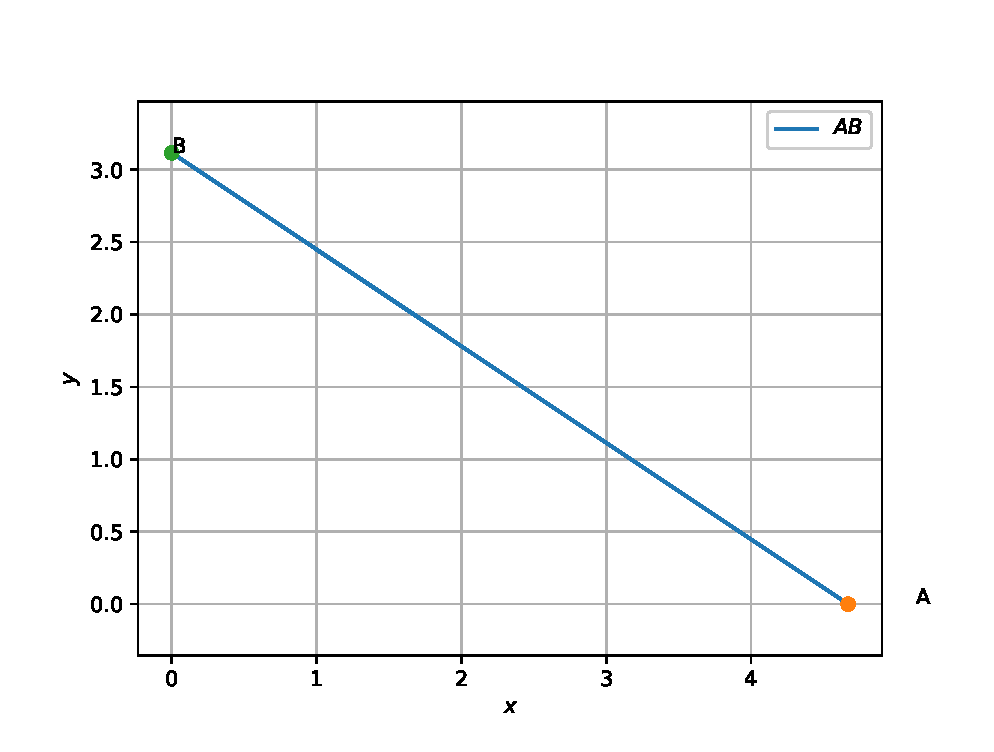
\includegraphics[width=\columnwidth]{./figures/plane_and_line1.eps}
	\caption{line1 }
	\label{fig:line1}
\end{figure}
\begin{lstlisting}
codes/plane_and_line1.py
\end{lstlisting}



\item put $\vec x \myvec{x\\0}$ in equation 
\begin{align}
\myvec{1 & -\frac{1}{5}}\myvec{x\\0} = 10
\\
x= 10
\end{align}
\\
put $\vec x \myvec{0\\y}$ in equation
\\
\begin{align}
\myvec{1 & -\frac{1}{5}}\myvec{0\\y} = 10
\\
y= -50
\\
\vec{P} = \myvec{10\\0}, \vec{Q} = \myvec{0\\-50}
\end{align}
\begin{figure}[!ht]
	\centering
	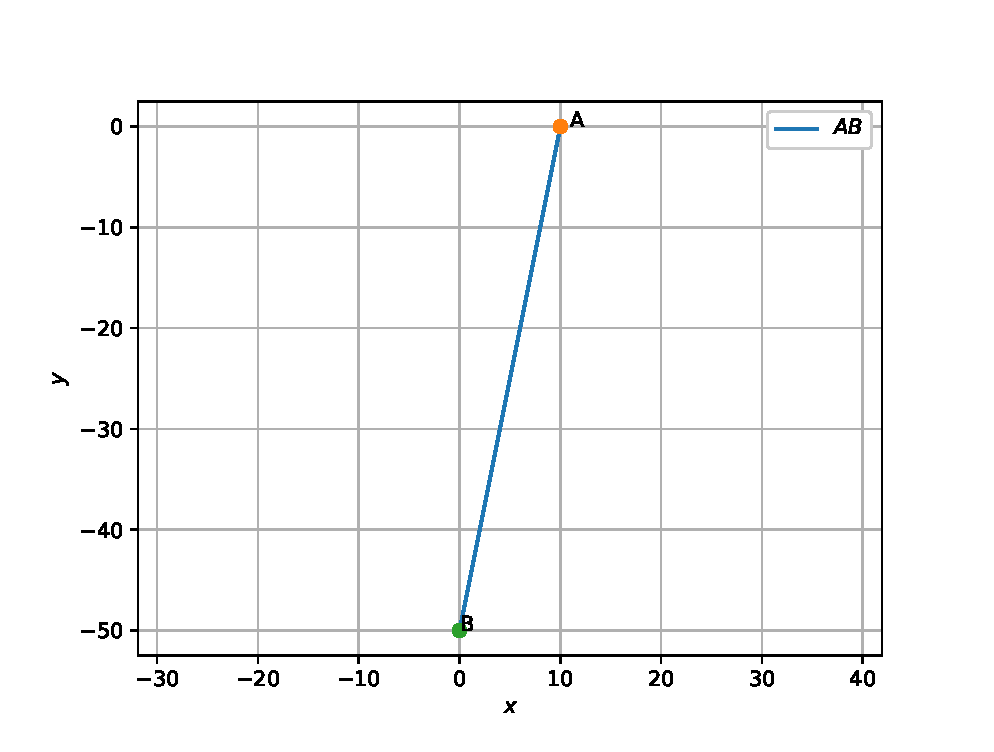
\includegraphics[width=\columnwidth]{./figures/plane_and_line2.eps}
	\caption{line2 }
	\label{fig:line2}
\end{figure}
\begin{lstlisting}
codes/plane_and_line2.py
\end{lstlisting}



\item put $\vec x \myvec{x\\0}$ in equation 
\begin{figure}[!ht]
	\centering
	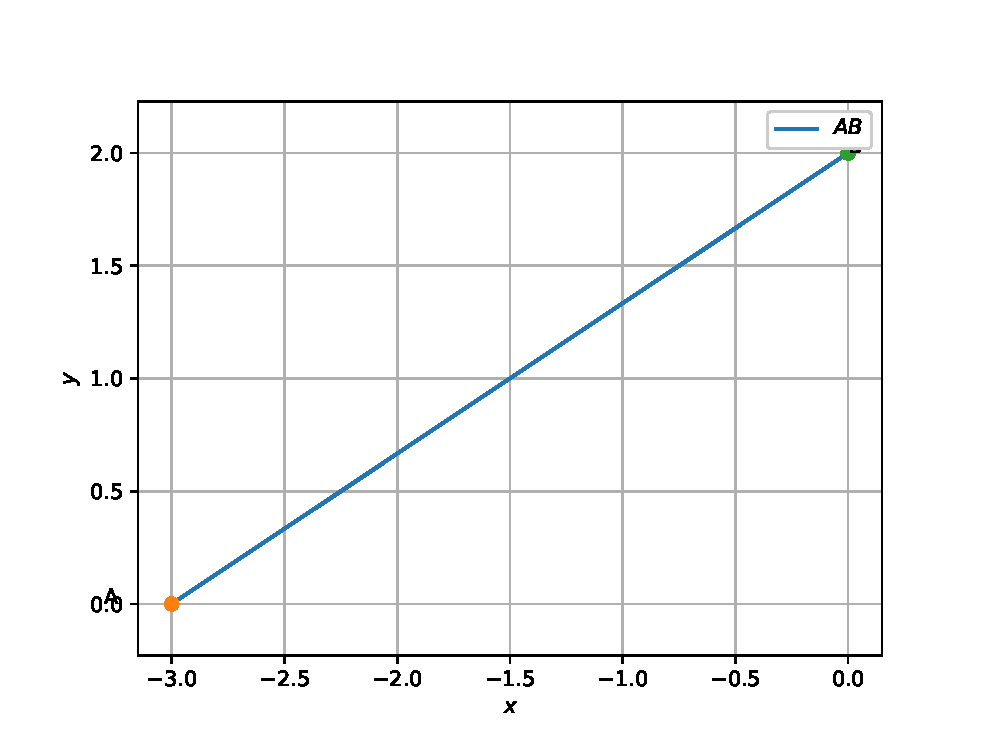
\includegraphics[width=\columnwidth]{./figures/plane_and_line3.eps}
	\caption{line3 }
	\label{fig:line3}
\end{figure}
\begin{lstlisting}
codes/plane_and_line3.py
\end{lstlisting}
\begin{align}
\myvec{-2 & 3}\myvec{x\\0} = 6
\\
x= -3
\end{align}
put $\vec x \myvec{0\\y}$ in equation
\\
\begin{align}
\myvec{-2 & 3}\myvec{0\\y} = 6
\\
y= 2
\\
\vec{P} = \myvec{-3\\0}, \vec{Q} = \myvec{0\\2}
\end{align}




\item there is no constant in the line equation thus it passes through the origin.
\\
put $\vec x \myvec{3\\y}$ in equation
\\
\begin{align}
\myvec{1 & -3}\myvec{3\\y} = 0
\\
y= 1
\\
\vec{P} = \myvec{0\\0}, \vec{Q} = \myvec{3\\1}
\end{align}
\begin{figure}[!ht]
	\centering
	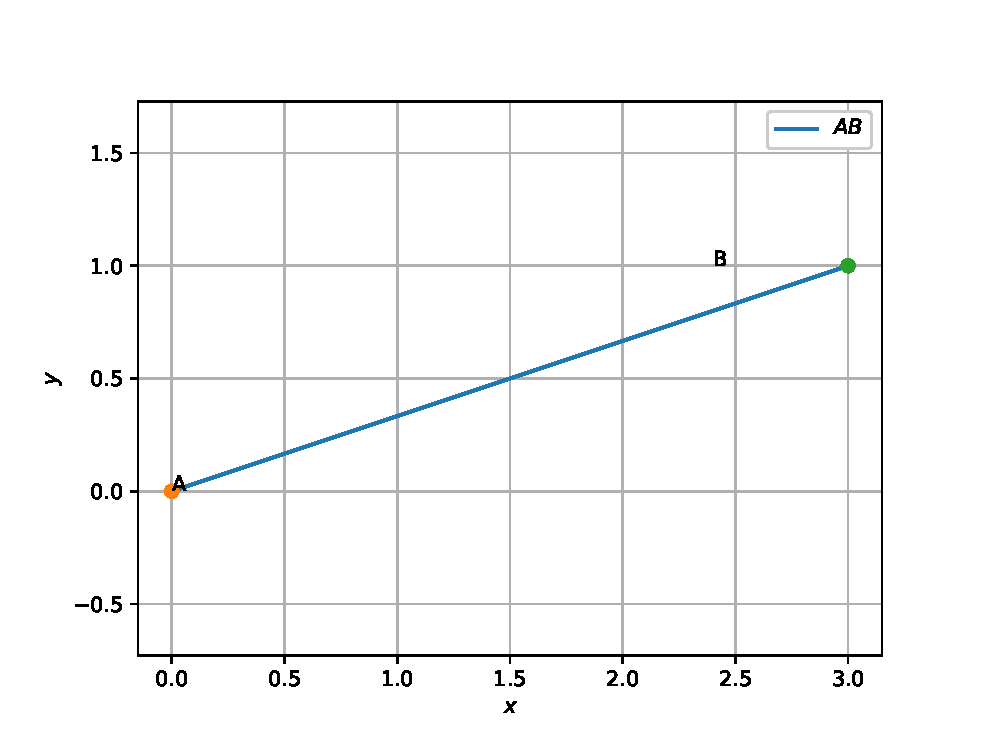
\includegraphics[width=\columnwidth]{./figures/plane_and_line4.eps}
	\caption{line4 }
	\label{fig:line4}
\end{figure}
\begin{lstlisting}
codes/plane_and_line4.py
\end{lstlisting}



\item there is no constant in the line equation thus it passes through the origin
\\
put $\vec x \myvec{1\\y}$ in equation
\\
\begin{align}
\myvec{2 & -1}\myvec{1\\y} = 0
\\
y= 1
\\
\vec{P} = \myvec{0\\0}, \vec{Q} = \myvec{1\\2}
\end{align}
\begin{figure}[!ht]
	\centering
	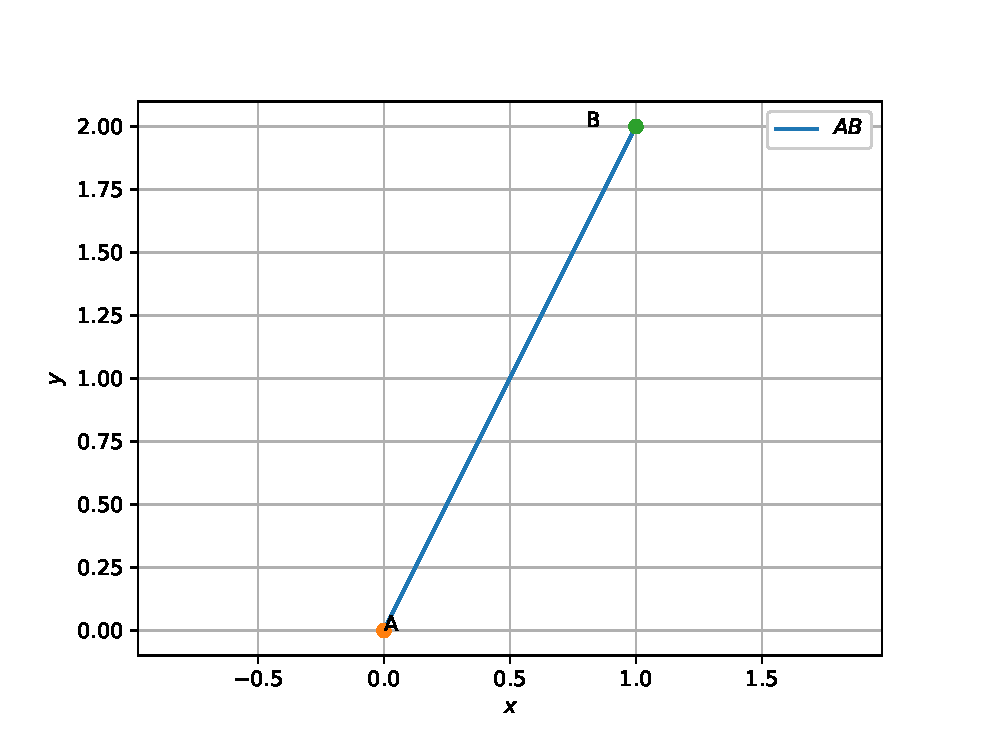
\includegraphics[width=\columnwidth]{./figures/plane_and_line5.eps}
	\caption{line5 }
	\label{fig:line5}
\end{figure}
\begin{lstlisting}
codes/plane_and_line5.py
\end{lstlisting}



\item put $\vec x \myvec{x\\0}$ in equation
\begin{figure}[!ht]
	\centering
	\includegraphics[width=\columnwidth]{./figures/plane_and_line6.eps}
	\caption{line6 }
	\label{fig:line6}
\end{figure}
\begin{lstlisting}
codes/plane_and_line6.py
\end{lstlisting} 
\begin{align}
\myvec{3 & 0}\myvec{x\\0} = -2
\\
x= -\frac{2}{3}
\end{align}
\\
we can see in this equation the  value of x coordinate does not depend on the y coordinate so we can say that it is parallel to the y-axis.





\item put $\vec x \myvec{x\\0}$ in equation 
\begin{align}
\myvec{0& 1}\myvec{0\\y} = 2
\\
y= 2
\end{align}
\\
we can see in this equation the  value of y coordinate does not depend on the x coordinate so we can say that it is parallel to the x-axis.
\begin{figure}[!ht]
	\centering
	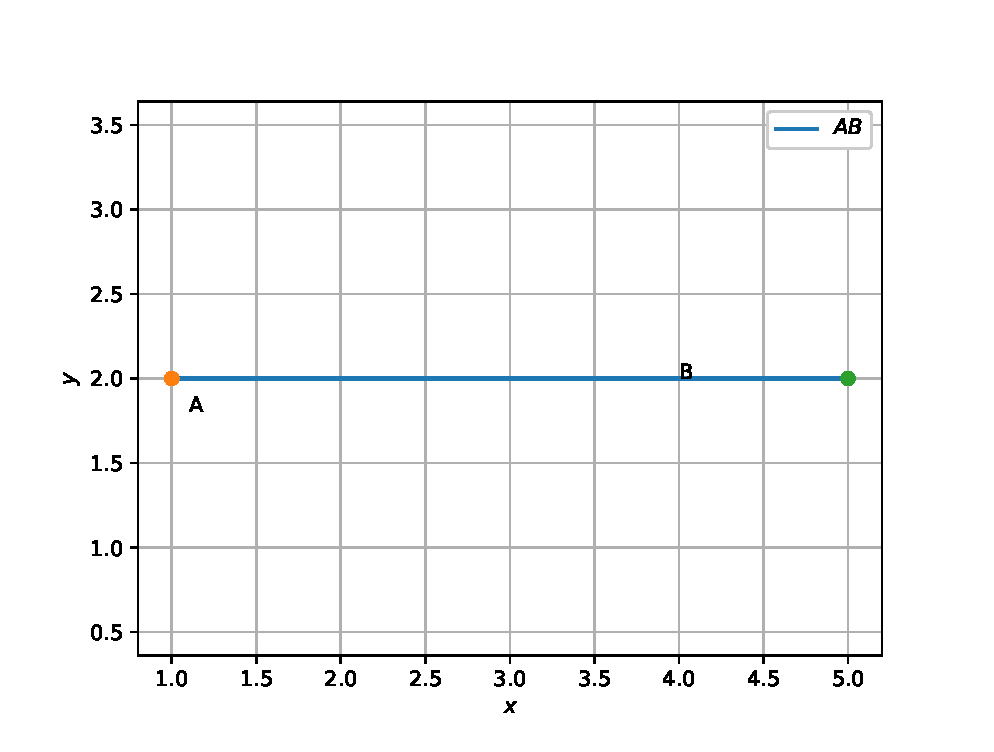
\includegraphics[width=\columnwidth]{./figures/plane_and_line7.eps}
	\caption{line7 }
	\label{fig:line7}
\end{figure}
\begin{lstlisting}
codes/plane_and_line7.py
\end{lstlisting} 



\item put $\vec x \myvec{x\\0}$ in equation 
\begin{align}
\myvec{2 & 0}\myvec{x\\0} = 5
\\
x= -\frac{5}{2}
\end{align}
\\
we can see in this equation the  value of x coordinate does not depend on the y coordinate so we can say that it is parallel to the y-axis.
\begin{figure}[!ht]
	\centering
	\includegraphics[width=\columnwidth]{./figures/plane_and_line8.eps}
	\caption{line8 }
	\label{fig:line8}
\end{figure}
\begin{lstlisting}
codes/plane_and_line8.py
\end{lstlisting} 
\end{enumerate}
\end{enumerate}